\subsection{Field Programmable Gate Arrays}
The computing hardware most people are familiar with is CPUs. Manufacturers incorporate them in every desktop pc, laptop, and most mobile devices. CPUs are very flexible and efficient- which is why they are the de facto standard for any computation task. In CPU computation, an integrated circuit (a processor) iteratively reads an instruction from a RAM module (in the form of encoded bits), performs the instruction, and then continues to read the next instruction. The instructions are not embedded in the circuit of the CPU itself.

FPGAs are different from CPUs, as they do not store the programs they execute in RAM- they instead configure them in the (highly parallel) logic of the circuit itself. Configuring an FPGA to execute a specific program entails loading a configuration file onto the hardware and restarting the FPGA such that it reconfigures its logic. The hardware will then perform the configured logic on the input it receives via IO pins. 

Because each logic cell performs logic independently, FPGAs can perform computations highly parallel and without delays from loading instructions. This computation process implies that FPGAs are very efficient at executing individual programs, specifically concurrent ones. Reconfiguring an FPGA is, however, a relatively expensive operation. Therefore, FPGAs are unsuitable for changing from program to program, as a CPU does when running an operating system.

FPGAs perform execution using lookup tables, registers, and special-purpose modules. These are physical modules that are on the circuit. In the next sections, we will discuss these modules.
\subsubsection{Lookup tables}
\begin{figure}
\centering
\begin{tabular}{|c|c|c|}
\hline
$p$ & $q$ & $p$ XOR $q$ \\ \hline
$F$ & $F$ & $F$       \\ \hline
$F$ & $T$ & $T$       \\ \hline
$T$ & $F$ & $T$       \\ \hline
$T$ & $T$ & $F$       \\ \hline
\end{tabular}
\caption{A truth table that shows the result of an XOR operation}
\label{fig:truth_table}
\end{figure}

\begin{figure}
\centering
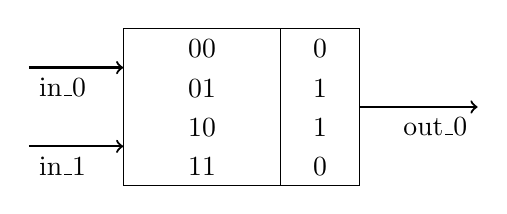
\begin{tikzpicture}
    \draw (0,0) rectangle (3,2);
    \draw (2, 0) -- (2, 2);
    \draw[thick,->] (-1.2,0.5) node[anchor=north west] {in\_1} -- (0,0.5);
    \draw[thick,->] (-1.2,1.5) node[anchor=north west] {in\_0} -- (0,1.5);
    
    \draw[thick,->] (3,1)  -- (4.5,1) node[anchor=north east] {out\_0};
    
    \draw[draw=white] (1,1.5)    node[anchor=south] {00};
    \draw[draw=white] (1,1)      node[anchor=south] {01};
    \draw[draw=white] (1,0.5)    node[anchor=south] {10};
    \draw[draw=white] (1,0)      node[anchor=south] {11};
    
    
    \draw[draw=white] (2.5,1.5)   node[anchor=south] {$0$};
    \draw[draw=white] (2.5,1)     node[anchor=south] {$1$};
    \draw[draw=white] (2.5,0.5)   node[anchor=south] {$1$};
    \draw[draw=white] (2.5,0)     node[anchor=south] {$0$};
\end{tikzpicture}
\caption{A Lookup Table (LUT) in which an XOR-operation is configured}
\label{fig:lookuptable}
\end{figure}

Any boolean logic formula can be expressed in the form of a truth table, such as in Figure \ref{fig:truth_table}. The leftmost column of a truth table specifies all possible combinations of $T$ and $F$ for all inputs; the rightmost column then specifies what output that specific logic function would give. Each distinct combination of $T$ and $F$ in the rightmost column corresponds to a different boolean formula. FPGAs execute logic in the form of Lookup Tables (LUTs), which model the evaluation of a truth table, but with ones and zeroes instead of $T$ and $F$: for every combination of ones and zeroes in the input, the LUT stores what output it should give. Vendor software can reconfigure these outputs. This way, any boolean formula with the appropriate number of variables can be implemented with a lookup table. Figure \ref{fig:lookuptable} shows a lookup table that has two input bits and one output bit. This lookup table is configured to perform an XOR-operation. Lookup tables can have input and output consisting of any number of bits, depending on the FPGA design.

\subsubsection{Registers}
\begin{figure}
\centering
\begin{tikzpicture}
    \draw (0,0) rectangle (1.5,2);
    \draw[-{Latex[length=5mm, open]}] (-1.2,0.5) node [anchor=north west] {$clock$} -- (0.5,0.5);
    \draw[-{Latex[length=3mm]}] (-1.2,1.5) node[anchor=east] {$D$} -- (0,1.5);
    
    \draw (-1.2,1.6) -- (-0.8,1.6);
    \draw (-0.8,1.6) -- (-0.5,1.5);
    \draw (-1.2,1.7) -- (-0.8,1.7);
    \draw (-0.8,1.7) -- (-0.5,1.5);

    
    \draw[-{Latex[length=3mm]}] (1.5,1) -- (2.7,1) node[anchor=west] {$Q$};
\end{tikzpicture}
\caption{Traditional representation of a register}
\label{fig:register}
\end{figure}

Programs require intermediate data storage to perform any computation that is more complex than finite logic or fixed-point calculations.

FPGAs use registers (or D flip-flops) for this purpose (see Figure \ref{fig:register}). Registers can store a small collection of bits, depending on the FPGA design. When a register's input $clock$ changes from 0 to 1, the contents of the register are replaced by the value of the input $D$, and the output $Q$ takes this value. The output stays constant until the clock changes from 0 to 1 again when D has a different value.

FPGAs usually have a global clock- a wire which signal constantly changes between 0 and 1 that is connected to all registers in the hardware. The frequency of this clock is such that all signals are guaranteed to be stable when the clock becomes 1. This stability is very convenient for programmers, who do not have to calculate the time it takes for a signal to propagate through a wire. The implication is that each circuit combining only lookup tables that end in the D-input of a register takes the same amount of time.

If the FPGA program has longer chains of lookup tables, then it takes longer for the output signal to stabilize. The vendor software accommodates for this by setting the global clock at a lower frequency. Since programs on FPGAs are highly parallel, there are likely some parts of the calculation that do not require a lower clock speed and can cause slowdown because of this. In these scenarios, adding registers to some parts of an FPGA program can improve performance if it allows the global clock speed to be higher.

\subsubsection{Logic Cells}
\begin{figure}
\centering
\begin{tikzpicture}
	%Register
    \draw (0,0) rectangle (1.5,2);
    \draw[-{Latex[length=5mm, open]}] (-1.2,-1) node [anchor=south east] {$clock$} -- (-1.2,0.5) -- (0.5,0.5);
    
    %Line from Register to MUX
    \draw[-{Latex[length=3mm]}] (1.5,1) -- (2.7,1) -- (2.7, 2.5) -- (3.7, 2.5);
    \draw (1.5, 1.1) -- (1.9, 1.1);
    \draw (1.5, 1.2) -- (1.9, 1.2);
    \draw (1.9, 1.1) -- (2.1, 1);
    \draw (1.9, 1.2) -- (2.1, 1);
    \draw (2.56,1) -- (2.7, 1.14);
    \draw (2.42,1) -- (2.7, 1.28);
    \draw (2.7, 2.36) -- (2.84, 2.5);
    \draw (2.7, 2.22) -- (2.98, 2.5);
    
    %LUT
    \draw (-5,2) rectangle (-2,4);
    \draw (-3, 2) -- (-3, 4);

    \draw[-{Latex[length=3mm]}] (-6.5,3) node[anchor=north west] {in} -- (-5,3);
	\draw (-6.5, 3.1) -- (-6.1, 3.1);
	\draw (-6.5, 3.2) -- (-6.1, 3.2);
	\draw (-6.1, 3.1) -- (-5.9, 3);
	\draw (-6.1, 3.2) -- (-5.9, 3);
    
    
    
    %Line from LUT to Register
    \draw[-{Latex[length=3mm]}] (-2,3)  -- (-1.1,3) -- (-1.1, 1.5) -- (0,1.5);
	
	\draw (-2,3.1) -- (-1.6,3.1);    
	\draw (-2,3.2) -- (-1.6,3.2);
	\draw (-1.6, 3.1) -- (-1.4, 3);
    \draw (-1.6, 3.2) -- (-1.4, 3);    

    \draw (-1.24, 3) -- (-1.1, 2.86);
    \draw (-1.38, 3) -- (-1.1, 2.72);
    \draw (-1.1, 1.64) -- (-0.96, 1.5);
    \draw (-1.1, 1.78) -- (-0.82, 1.5);
    
    
    %LUT keys
    \draw[draw=white] (-4,3.25) node[anchor=south] {$0000$};
    \draw[draw=white] (-4,2.75) node[anchor=south] {$\cdots$};
    \draw[draw=white] (-4,2.25) node[anchor=south] {$1111$};
    
    %LUT values
    \draw[draw=white] (-2.5,3.25) node[anchor=south] {$x_0$};
    \draw[draw=white] (-2.5,2.75) node[anchor=south] {$\cdots$};
    \draw[draw=white] (-2.5,2.25) node[anchor=south] {$x_n$};
    
    %Line from LUT to MUX
    \draw[-{Latex[length=3mm]}] (-2,3)  -- (3.7,3);
    
    %MUX
    \draw (3.7, 3.5) -- (3.7, 1.5) -- (4.7, 2) -- (4.7, 3) -- cycle;
    
    %M
    \draw[-{Latex[length=3mm]}] (2.2, 0.5) node[anchor=north west] {$m$} --(3.2, 0.5) -- (3.2, 2) -- (3.7, 2);
    
    %\draw[-{Latex[length=3mm]}] (4.7, 3) -- (6.2, 3) node[anchor = north east] {out\_0};
    %\draw[draw=white] (4.7, 2.5) -- (6.2, 2.5) node[anchor = north east] {$\cdots$};
    
    \draw[-{Latex[length=3mm]}] (4.7, 2.5) -- (6.2, 2.5) node[anchor = north east] {out};
    \draw (4.7, 2.6) -- (5.1, 2.6);
    \draw (4.7, 2.7) -- (5.1, 2.7);
    \draw (5.1, 2.6) -- (5.3, 2.5);
    \draw (5.1, 2.7) -- (5.3, 2.5);      

    
\end{tikzpicture}
\caption{An $n$-input logic cell. $x_k$ and $m$ must be configured for any $0 \leq k \leq n$}
\label{fig:logiccell}
\end{figure}

A typical logic cell is a combination of one or more lookup tables, a register, and a MUX (a 3-input gate that outputs a copy of the first or second input, depending on the value of the third input).  The contents of the lookup tables can be configured to perform any logic operation, and the value of the third MUX-input can be configured to specify whether the computation is synchronous or asynchronous. A logic cell is shown in Figure \ref{fig:logiccell}. Unfortunately for us, vendors have different logic cell designs, meaning we cannot generalize this example.

FPGA manufacturers often group Logic cells in Configurable Logic Blocks (CLB) that make hardware production, placement, and routing (Section \ref{sec:compilation}) easier.
 
The main building blocks of FPGAs are CLBs that are connected via routing fabric. These are responsible for most of the computation of FPGA programs. FPGAs can have additional modules such as RAM and Digital Signal Processors that optimize storage and specialized arithmetic, respectively. Each of these modules' functionality could also be performed by a collection of logic cells at the cost of performance. In this research, we will only consider CLBs.

\subsubsection{Routing}
A single logic cell can only perform simple programs such as logic gates. The FPGA needs to connect different logic cells to perform any kind of logic operation, dependent on what program it needs to execute. The way logic cells and other modules are connected on an a physical FPGA in a specific configuration is called the \textbf{routing} of an FPGA. On the most basic level, FPGAs perform routing with configurable switches. These are tiny modules on an FPGA board that is connected with $>2$ wires, and can be configured to block signals from specific wires; the other wires can then send- and receive signals.

\subsubsection{Pins}
To supply the FPGA with input and to allow it to provide output, an FPGA is equipped with a set of metal pins. Each of those pins is connected with a wire on the FPGA board. Each pin can be used for either input or output, depending on the configured program. For example, an FPGA used to control an electric stepper motor will receive input with the requested motor speed and direction and will output power to specific electromagnets that need to be activated.

\subsubsection{Compilation}
\label{sec:compilation}
To program an FPGA, an engineer has to specify a hardware design that describes the semantics of the program. They write these hardware designs in a Hardware Description Language (HDL). Commonly used languages for this purpose are VHDL and Verilog. They specify on an abstract level what functionality the program should have, preferably in a modular structure to improve maintainability.

The software then needs to translate this abstract description to a description of logic, data storage, and how they are connected. This process depends on the available hardware components on a physical FPGA and is thus hardware-specific. This process is called \textbf{synthesis}. Although synthesis is a polynomial problem, it can still take minutes to perform for some programs\cite{BDDSynthesis, pistorius2007benchmarking}.

The next step in the compilation process is \textbf{placement}. The software maps each LUT, register, and other component to a physical place on the FPGA. The software can place components closer together to optimize the speed or can place components further apart to increase the probability routes can be found. Finding the optimal placement for speed is a proven NP-hard problem.

The last step in the compilation process is \textbf{routing}. State-of-the-art FPGA compilation pipelines perform this step sequentially after placement\cite{alhyari2019}. With the components locked in place, the software attempts to find a configuration of routing switches such that each connection that the synthesis requires is made. Finding the optimal routes for speed is also an NP-hard problem. However, finding any matching routing configuration is an NP problem.

\begin{figure}[h]
\centering
\begin{tabular}{|p{0.97\textwidth}|}
\hline
Note that place \& route of an FPGA \textit{program} as described here is a very similar problem to placement of an unconfigured virtual FPGA, which is part of this research. A conventional place \& route algorithm could (with some minor modification) place a virtual FPGA model with all its components on a concrete FPGA, resulting in a mapping we could use for emulation.

The problem with this approach is that state-of-the art place \& route pipelines perform these algorithms sequentially: they perform placement based on speed- and routeability heuristics without guarantee that the placement can indeed be routed\cite{alhyari2019}. With placement of FPGA programs this is not a problem. Entire FPGAs, however, can have dense collections of components that can severely impact routeability.

Not using well-founded placement algorithms based on heuristics will undoubtedly have an adverse impact on the speed of our placement. However, we can use the hierarchical structure of an FPGA for significant improvements that could not be obtained with placement of FPGA programs.
\\\hline
\end{tabular}
\end{figure}



\begin{figure}
    \centering
\begin{tikzpicture}
    \draw (0,0) rectangle (3,2);
    \draw (2, 0) -- (2, 2);
    \draw[thick,->] (-1.2,0.5) node[anchor=north west] {in\_2} -- (0,0.5);
    \draw[thick,->] (-1.2,1.5) node[anchor=north west] {in\_1} -- (0,1.5);
    
    \draw[thick,->] (3,1)  -- (4,1) node[anchor=north west] {out\_1};
    
    \draw[draw=white] (1,1.5)    node[anchor=south] {00};
    \draw[draw=white] (1,1)      node[anchor=south] {01};
    \draw[draw=white] (1,0.5)    node[anchor=south] {10};
    \draw[draw=white] (1,0)      node[anchor=south] {11};
    
    
    \draw[draw=white] (2.5,1.5)     node[anchor=south] {$x_0$};
    \draw[draw=white] (2.5,1)       node[anchor=south] {$x_1$};
    \draw[draw=white] (2.5,0.5)     node[anchor=south] {$x_2$};
    \draw[draw=white] (2.5,0)       node[anchor=south] {$x_3$};
    
    

    \draw (8,-1.5) rectangle (11,2);
    \draw (10, -1.5) -- (10, 2);
	
	\draw[thick,->] (6.8,1.9) node[anchor=north west] 	{$x_0$} -- (8,1.9);
	\draw[thick,->] (6.8,1.3) node[anchor=north west] 	{$x_1$} -- (8,1.3);
	\draw[thick,->] (6.8,0.7) node[anchor=north west] 	{$x_2$} -- (8,0.7);
	\draw[thick,->] (6.8,0.1) node[anchor=north west] 	{$x_3$} -- (8,0.1);
	\draw[thick,->] (6.8,-0.5) node[anchor=north west] 	{in\_1} -- (8,-0.5);
    \draw[thick,->] (6.8,-1.1) node[anchor=north west] 	{in\_2} -- (8,-1.1);

    
    \draw[thick,->] (11,1)  -- (12,1) node[anchor=north west] {out\_1};
    
    \draw[draw=white] (9,1.5)       node[anchor=south] {000000};
    \draw[draw=white] (9,1)         node[anchor=south] {000001};
    \draw[draw=white] (9,0.5)       node[anchor=south] {000010};
	\draw[draw=white] (9,0)         node[anchor=south] {$\cdots$};
    \draw[draw=white] (9,-0.5)      node[anchor=south] {111101};
    \draw[draw=white] (9,-1) 	    node[anchor=south] {111110};
    \draw[draw=white] (9,-1.5)      node[anchor=south] {111111};
    
    
    
    \draw[draw=white] (10.5,1.5)         node[anchor=south] {$0$};
    \draw[draw=white] (10.5,1)           node[anchor=south] {$0$};
    \draw[draw=white] (10.5,0.5)         node[anchor=south] {$0$};
	\draw[draw=white] (10.5,0)           node[anchor=south] {$\cdots$};
	\draw[draw=white] (10.5,-0.5)        node[anchor=south] {$1$};
	\draw[draw=white] (10.5,-1)          node[anchor=south] {$1$};
	\draw[draw=white] (10.5,-1.5)        node[anchor=south] {$1$};
    
    
    \draw[vecArrow] (5.5,1) -- (6.5,1);

\end{tikzpicture}
    \caption{Simulation of an FPGA: the programming of the virtual FPGA is reflected in additional input of the actual FPGA. The value of $x$ in the simulation is identical to the configuration of the program to be simulated.}
    \label{fig:simulation}
\end{figure}